% Provenance (never printed): cycle 2 "Explorer les organisations du monde ---
% identifier des paysages" (littoraux, massifs montagneux, campagnes, villes),
% see sources/book1/PROVENANCE.md. Book 1, grade 1, chapter 2.
\chapter{身边的景观}\label{ch:g1:landscapes-around-us}

米娅和爷爷沿着村子后面的小山
一路走到了山顶。他们在草地上坐下歇口气，
然后向远处望去。脚下，村子的红色屋顶挤在教堂周围。一条
河在绿色和黄色的田野之间蜿蜒流淌，从一座桥下穿过。
隔壁的山上有一片黑色的森林。再远再远的地方，在陆地的尽头，
有一条细细的蓝线。

“那是大海，”爷爷说。

米娅从山顶上能看到的一切，无论远近，都是
\omterm{def:g1:landscapes-around-us:landscape}{景观}。

\begin{omfigure}
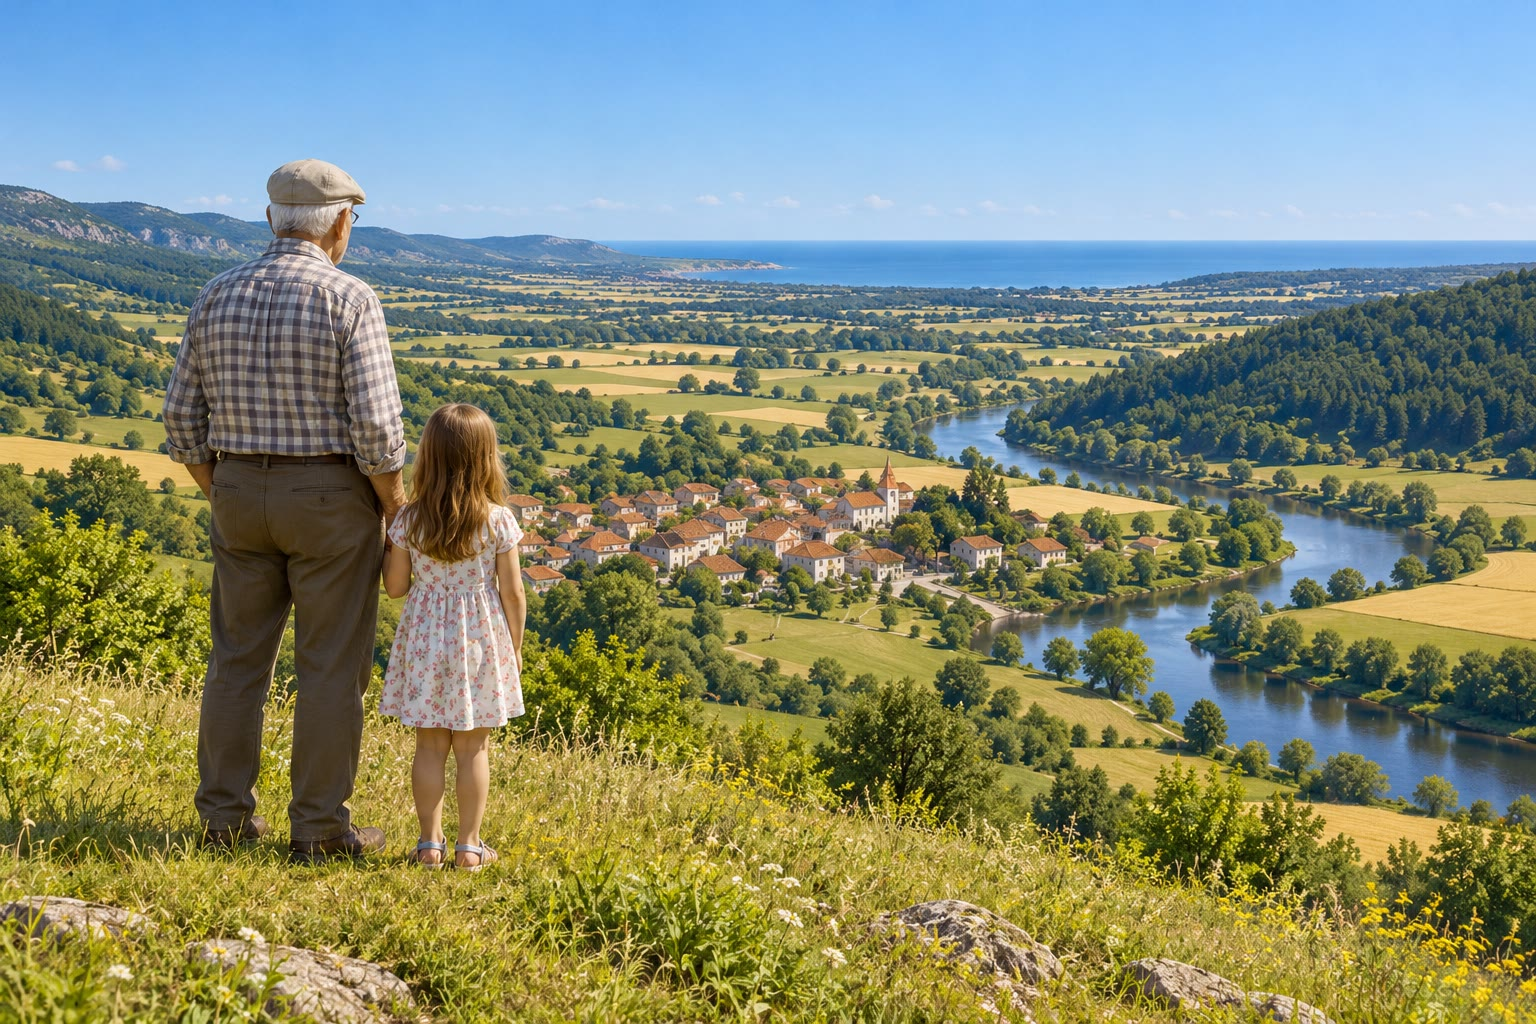
\includegraphics[width=0.72\linewidth]{images/book1/ai/g1-hilltop-view.jpg}

{\small 从山顶望去，我们能看到一整片\omterm{def:g1:landscapes-around-us:landscape}{景观}。}
\end{omfigure}

\section{什么是景观？}

\begin{definition}[景观]\label{def:g1:landscapes-around-us:landscape}
站在某处，一眼望去，我们能看到的陆地上的一切，就是\emph{景观}\index{景观}：
从所站之处直到遥远的地平线，地面的形状、
水、植物，以及人们建造的东西。
\end{definition}

\omterm{def:g1:landscapes-around-us:landscape}{景观}既有近处的部分，也有远处的部分。离我们最近的部分
位于我们所见画面的底部，它看起来很大，我们能看清它的
细节。远处的部分在顶部，靠近天空，它看起来很小，
颜色也很淡。

\begin{omfigure}
\begin{tikzpicture}[x=1cm, y=1cm]
  \fill[ocBlue!12] (0,0) rectangle (10,5);
  % background: far hills
  \fill[black!18] (0,3.0) -- (1.5,3.6) -- (3,3.3) -- (5,3.9) -- (7,3.4) -- (8.5,3.8) -- (10,3.3) -- (10,2.9) -- (0,2.9) -- cycle;
  % middle: hills and fields
  \fill[green!35!omLithAlluv] (0,1.6) -- (2,2.4) -- (4,2.1) -- (6,2.7) -- (8,2.2) -- (10,2.5) -- (10,1.5) -- (0,1.5) -- cycle;
  \fill[green!25!omLithAlluv] (0,1.5) rectangle (10,2.95);
  \fill[green!35!omLithAlluv] (0,2.95) -- (2,3.1) -- (4,2.95) -- (6,3.25) -- (8,3.0) -- (10,3.1) -- (10,2.9) -- (0,2.9) -- cycle;
  \foreach \x in {5.6,5.9,6.2} \fill[red!55] (\x,2.25) -- ++(0.12,0.15) -- ++(0.12,-0.15) -- cycle;
  \foreach \x in {5.6,5.9,6.2} \fill[white] (\x+0.03,2.1) rectangle ++(0.18,0.15);
  % foreground
  \fill[green!55!black!60] (0,0) rectangle (10,1.5);
  \foreach \x in {0.8,2.1,8.6} {
    \fill[brown!70!black] (\x-0.06,0.4) rectangle (\x+0.06,0.9);
    \fill[green!45!black] (\x,1.15) circle (0.38);
  }
  % band borders and labels
  \draw[white, line width=1pt, dashed] (0,1.5) -- (10,1.5);
  \draw[white, line width=1pt, dashed] (0,2.95) -- (10,2.95);
  \node[font=\small\bfseries, fill=white, fill opacity=0.8, text opacity=1, inner sep=2pt] at (5,0.6) {前景：近、大、细节多};
  \node[font=\small\bfseries, fill=white, fill opacity=0.8, text opacity=1, inner sep=2pt] at (2.7,2.2) {中景};
  \node[font=\small\bfseries, fill=white, fill opacity=0.8, text opacity=1, inner sep=2pt] at (5,4.4) {背景：远、小、颜色淡};
\end{tikzpicture}

{\small \omterm{def:g1:landscapes-around-us:landscape}{景观}分为三层：底部是前景，
中间是中景，与天空相接的是背景。}
\label{fig:g1:landscapes-around-us:bands}
\end{omfigure}

\section{地面的形状}

地面并不是到处都是平的。在有些地方，它高高地耸入
天空；在另一些地方，它向下陷成长长的洼地；还有些地方，
放眼望去都是平坦的。我们给每一种形状起一个名字。

\begin{definition}[地貌]\label{def:g1:landscapes-around-us:landform}
\emph{地貌}\index{地貌}是地表的一种形状。
\begin{itemize}
  \item \emph{山}\index{山}是非常高的地貌，坡度陡
        峭；山顶叫作山峰。最高的山，即使在夏天，山顶也有
        积雪。
  \item \emph{丘陵}\index{丘陵}是高出周围土地的地貌，
        比山矮，形状也更圆润。
  \item \emph{山谷}\index{山谷}是位于丘陵或山之间的又长又低的洼地，
        谷底常常有一条河。
  \item \emph{平原}\index{平原}是宽阔、平坦、低矮的一片土地。
\end{itemize}
\end{definition}

\begin{omfigure}
\begin{tikzpicture}[x=1cm, y=1cm]
  \fill[ocBlue!10] (0,0) rectangle (12.4,4.6);
  % sea
  \fill[omSea] (10.2,0) rectangle (12.4,0.55);
  % land profile: mountains, valley, hill, plain, coast
  \fill[omLithAlluv!80!green] (0,0) -- (0,2.2) -- (0.9,3.3) -- (1.5,3.0) -- (2.2,4.1)
     -- (2.9,2.6) -- (3.6,1.2) -- (3.9,0.9) -- (4.2,1.2) -- (5.0,2.0) -- (5.7,2.2)
     -- (6.4,1.6) -- (7.0,0.95) -- (8.0,0.8) -- (9.5,0.7) -- (10.2,0.6) -- (10.4,0.55)
     -- (10.4,0) -- cycle;
  \draw[black!60, line width=0.6pt] (0,2.2) -- (0.9,3.3) -- (1.5,3.0) -- (2.2,4.1)
     -- (2.9,2.6) -- (3.6,1.2) -- (3.9,0.9) -- (4.2,1.2) -- (5.0,2.0) -- (5.7,2.2)
     -- (6.4,1.6) -- (7.0,0.95) -- (8.0,0.8) -- (9.5,0.7) -- (10.2,0.6) -- (10.4,0.55);
  % snow caps
  \fill[white, draw=black!50, line width=0.3pt] (1.95,3.72) -- (2.2,4.1) -- (2.45,3.72) -- (2.3,3.78) -- (2.2,3.68) -- (2.08,3.78) -- cycle;
  \fill[white, draw=black!50, line width=0.3pt] (0.72,3.08) -- (0.9,3.3) -- (1.05,3.15) -- (0.9,3.12) -- cycle;
  % river in the valley
  \fill[omSea!90!black] (3.75,0.92) rectangle (4.05,0.98);
  % lake on the plain
  \fill[omSea] (7.6,0.82) ellipse (0.5 and 0.07);
  % village on the plain
  \foreach \x in {8.6,8.85,9.1} {
    \fill[white, draw=black!50, line width=0.3pt] (\x,0.74) rectangle ++(0.18,0.16);
    \fill[red!60] (\x-0.02,0.9) -- ++(0.11,0.12) -- ++(0.11,-0.12) -- cycle;
  }
  % labels
  \node[font=\small, above] at (2.2,4.12) {山};
  \node[font=\small, above] at (5.6,2.25) {丘陵};
  \node[font=\small] at (3.9,1.85) {山谷};
  \node[font=\small, above] at (8.2,1.5) {平原};
  \draw[black!60, thin] (8.2,1.5) -- (8.2,0.85);
  \node[font=\small, align=center] at (11.3,1.4) {海};
  \node[font=\scriptsize, below=2pt, fill=white, fill opacity=0.8, text opacity=1, inner sep=1pt] at (7.6,0.35) {湖泊};
  \draw[black!60, thin] (7.6,0.45) -- (7.6,0.78);
  \node[font=\scriptsize, below=2pt, fill=white, fill opacity=0.8, text opacity=1, inner sep=1pt] at (10.3,0.35) {海岸};
  \node[font=\scriptsize, fill=white, fill opacity=0.8, text opacity=1, inner sep=1pt] at (3.9,0.2) {河流};
  \draw[black!60, thin] (3.9,0.32) -- (3.9,0.88);
\end{tikzpicture}

{\small 从山脉到大海，从侧面看到的陆地形状
（图中高度比实际高得多）。}
\label{fig:g1:landscapes-around-us:profile}
\end{omfigure}

\begin{omfigure}
\begin{minipage}[b]{0.49\linewidth}\centering
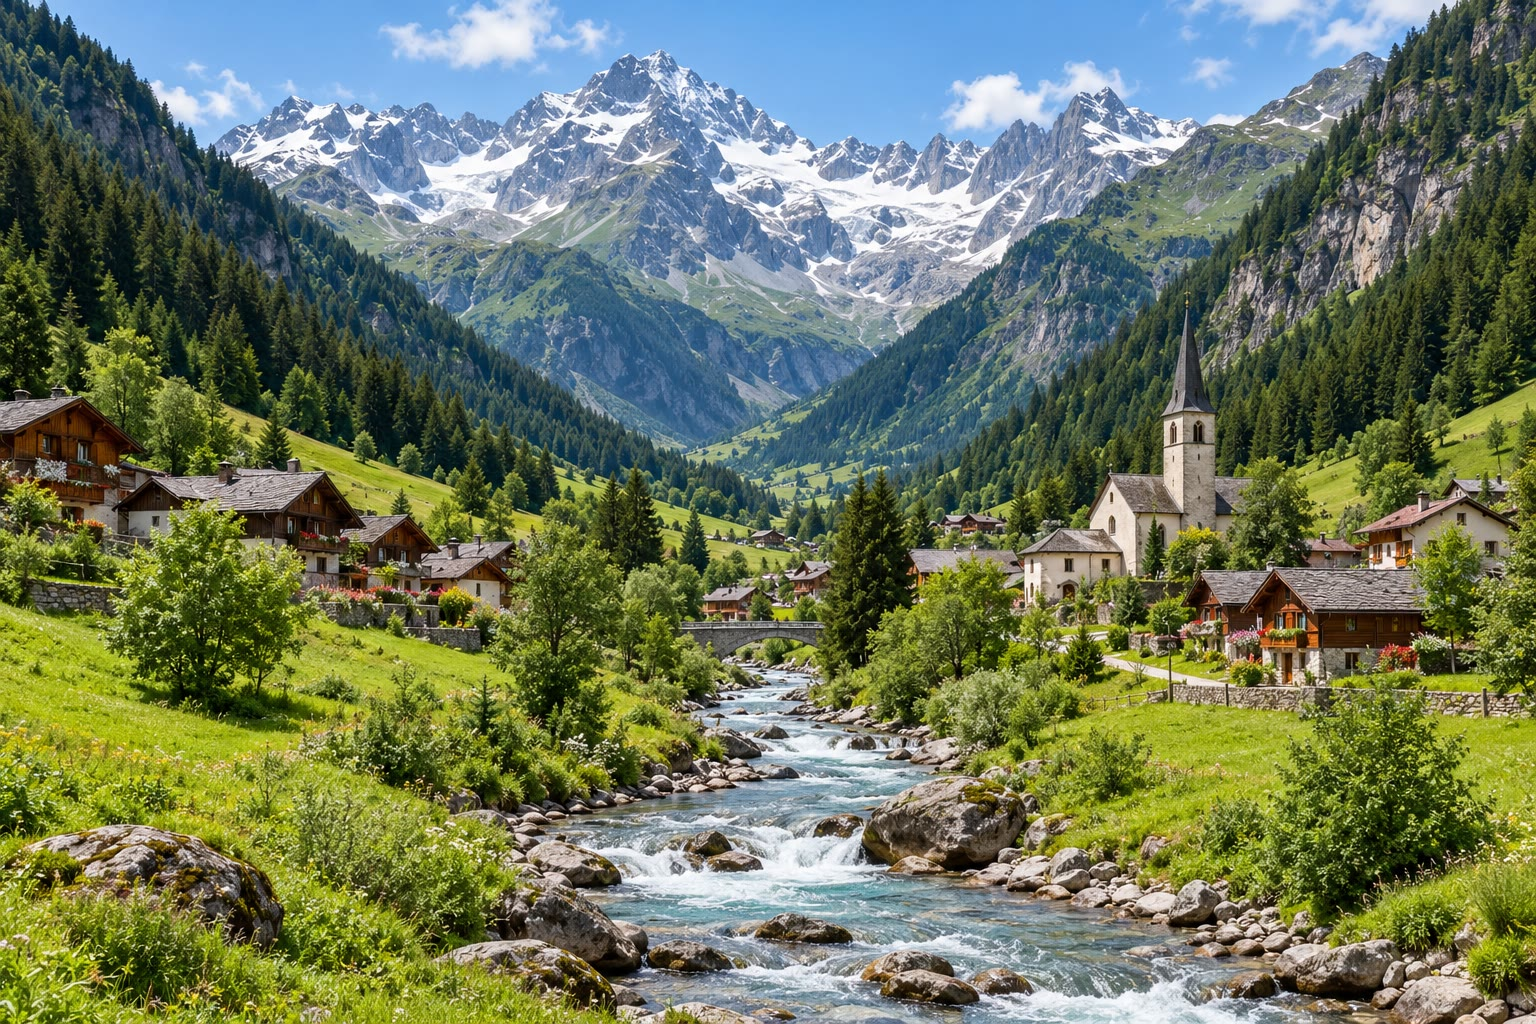
\includegraphics[width=\linewidth]{images/book1/ai/g1-mountain-village.jpg}

{\small 山脉，以及\omterm{def:g1:landscapes-around-us:landform}{山谷}中的一个村庄。}
\end{minipage}\hfill
\begin{minipage}[b]{0.49\linewidth}\centering
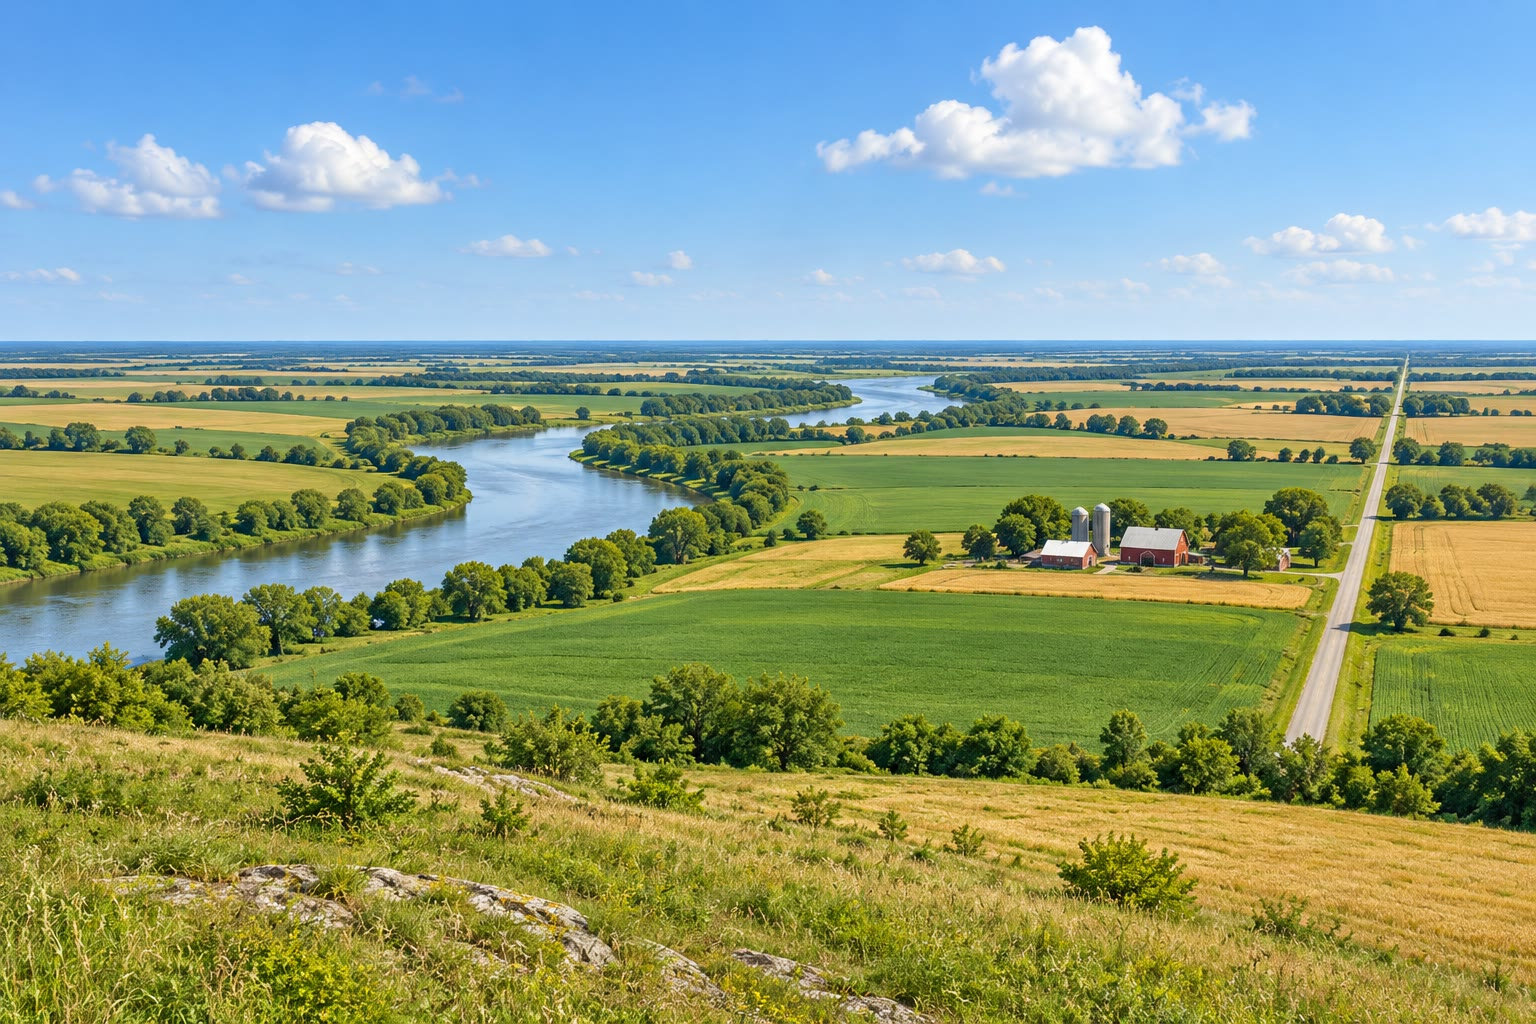
\includegraphics[width=\linewidth]{images/book1/ai/g1-plain-river.jpg}

{\small \omterm{def:g1:landscapes-around-us:landform}{平原}，有\omterm{def:g1:landscapes-around-us:water}{河流}和田地。}
\end{minipage}
\end{omfigure}

\begin{example}[山还是丘陵？]\label{ex:g1:landscapes-around-us:mountain-hill}
\omterm{def:g1:landscapes-around-us:landform}{丘陵}变成山并没有确切的高度。我们看的是
形状：山高而陡，多岩石，有时山顶有雪；
\omterm{def:g1:landscapes-around-us:landform}{丘陵}则较矮、较圆，常被草地、田地或
树林覆盖，人们很快就能走到它的山顶。
\end{example}

\section{景观中的水}

水是大多数\omterm{def:g1:landscapes-around-us:landscape}{景观}的一部分。它从\omterm{def:g1:landscapes-around-us:landform}{丘陵}和
山脉流下，汇集于洼地，最终流入大海。

\begin{definition}[景观中的水]\label{def:g1:landscapes-around-us:water}
\emph{河流}\index{河流}是在长长的河道中
一直流动的水，从较高处流向湖泊或大海。
\emph{湖泊}\index{湖泊}是被陆地包围的大片水体。
\emph{海岸}\index{海岸}是陆地与大海相接的地方。
\end{definition}

\begin{omfigure}
\begin{minipage}[b]{0.49\linewidth}\centering
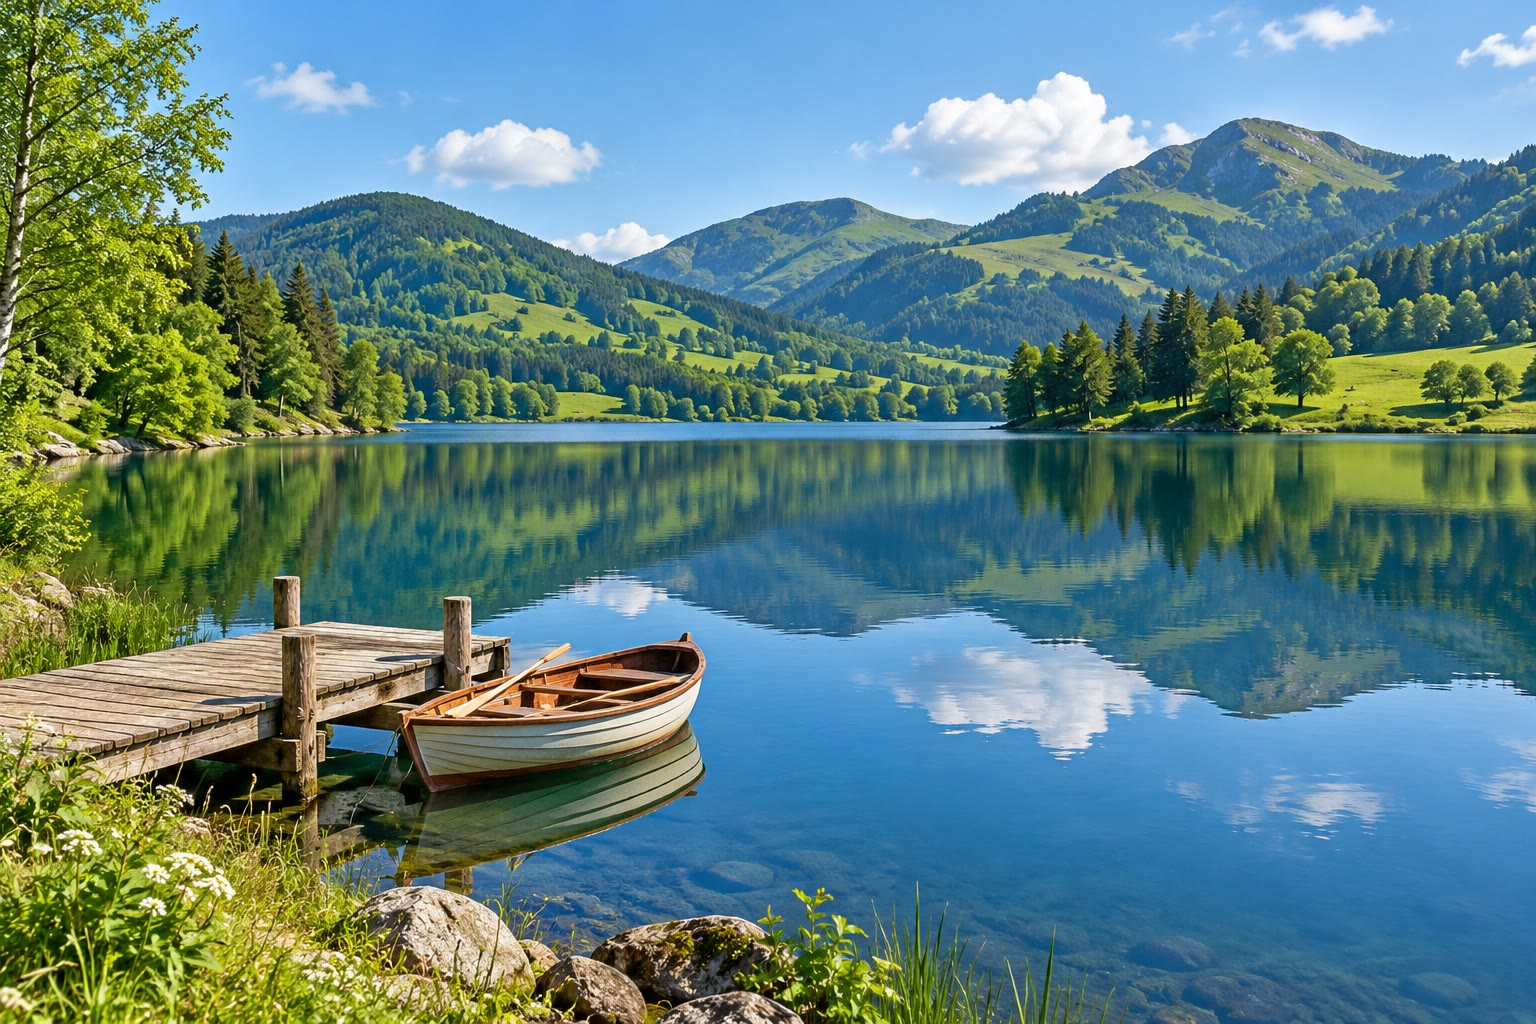
\includegraphics[width=\linewidth]{images/book1/ai/g1-lake-hills.jpg}

{\small \omterm{def:g1:landscapes-around-us:landform}{丘陵}间的\omterm{def:g1:landscapes-around-us:water}{湖泊}。}
\end{minipage}\hfill
\begin{minipage}[b]{0.49\linewidth}\centering
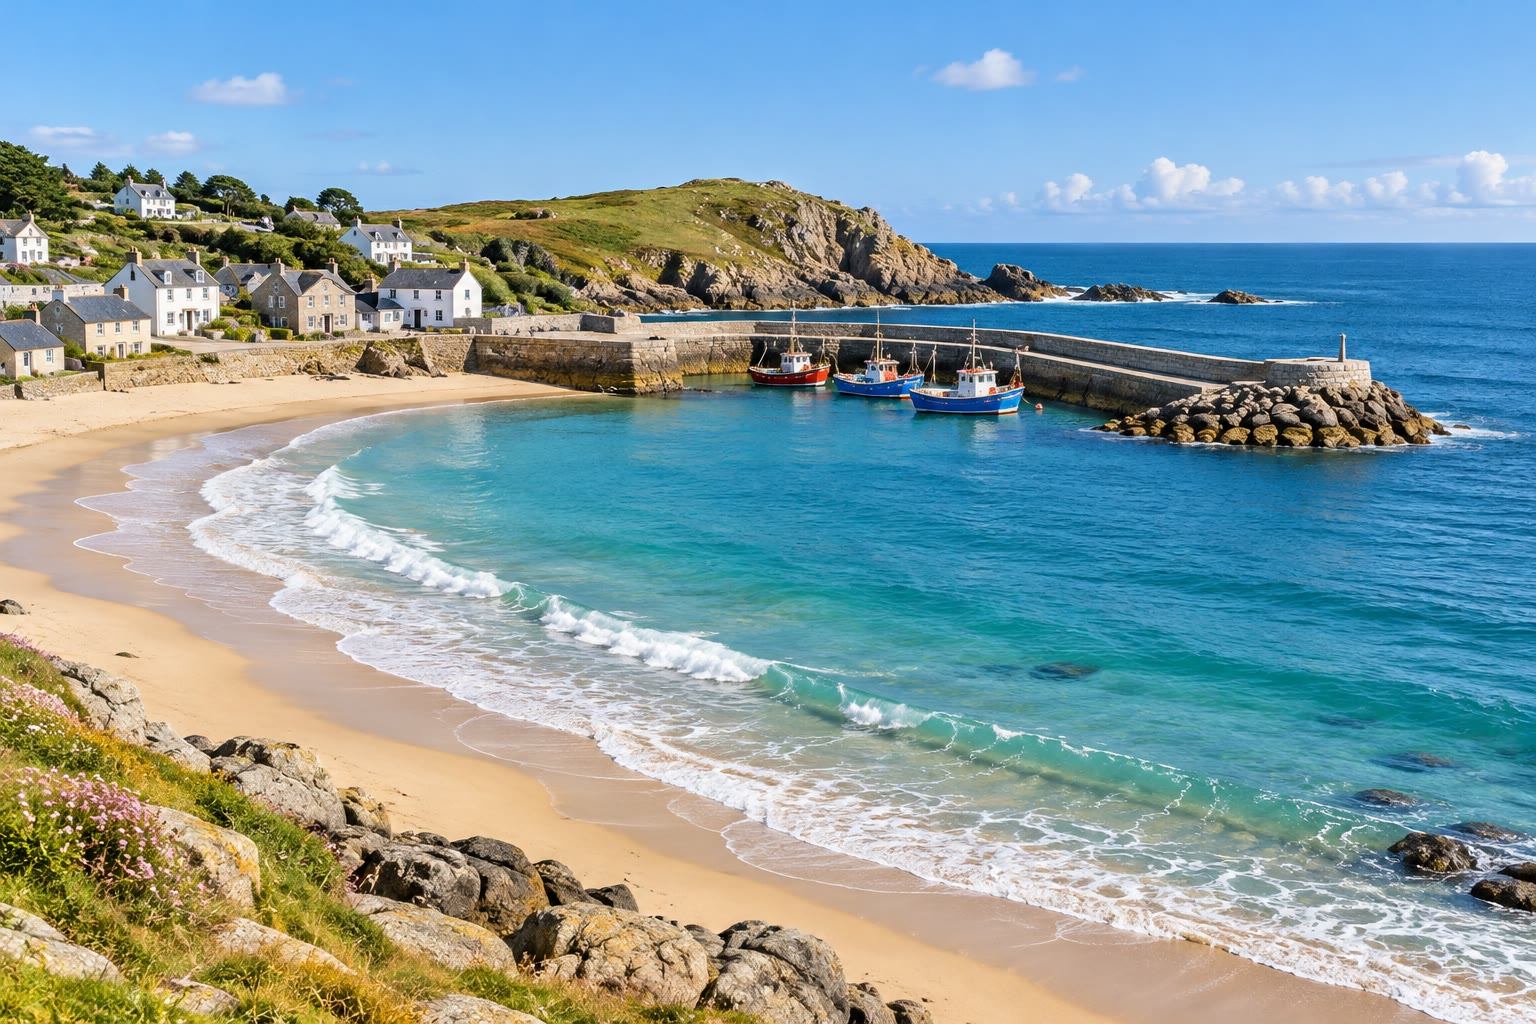
\includegraphics[width=\linewidth]{images/book1/ai/g1-coast-harbour.jpg}

{\small \omterm{def:g1:landscapes-around-us:water}{海岸}：海滩、岩石和港口。}
\end{minipage}
\end{omfigure}

\begin{remark}[水总是向低处流]\label{rem:g1:landscapes-around-us:downhill}
\omterm{def:g1:landscapes-around-us:water}{河流}总是从高处流向低处。这就是为什么
\omterm{def:g1:landscapes-around-us:water}{河流}沿\omterm{def:g1:landscapes-around-us:landform}{山谷}底部流动，最终流入\omterm{def:g1:landscapes-around-us:water}{湖泊}
或大海，因为它们都比周围的陆地低。
\end{remark}

\section{自然要素与人工要素}

\omterm{def:g1:landscapes-around-us:landscape}{景观}中的一些部分在人类到来之前就已存在：山脉、
\omterm{def:g1:landscapes-around-us:water}{河流}、森林。另一些部分则是人类建造的：房屋、道路、
桥梁、田地。

\begin{definition}[自然要素与人工要素]\label{def:g1:landscapes-around-us:natural-built}
\omterm{def:g1:landscapes-around-us:landscape}{景观}中的\emph{自然要素}\index{自然要素}是指
非人类建造的部分：山、\omterm{def:g1:landscapes-around-us:water}{河流}、\omterm{def:g1:landscapes-around-us:water}{湖泊}、森林、海滩。
\omterm{def:g1:landscapes-around-us:landscape}{景观}中的\emph{人工要素}\index{人工要素}是指由人
建造或改造的部分：房屋、道路、桥梁、港口、田地、花园。
\end{definition}

\begin{omfigure}
\begin{tikzpicture}[x=1cm, y=1cm]
  \node[draw=omDef!80!black, fill=omDef!10, rounded corners, text width=5.2cm,
        align=left, minimum height=3.2cm, anchor=north] (n) at (0,0)
    {\textbf{自然}\\[2pt] 山 \\ 丘陵 \\ 山谷 \\ 河流 \\ 湖泊 \\ 森林 \\ 海滩};
  \node[draw=omMeth!80!black, fill=omMeth!10, rounded corners, text width=5.2cm,
        align=left, minimum height=3.2cm, anchor=north] (b) at (6,0)
    {\textbf{人工建造}\\[2pt] 房屋 \\ 教堂 \\ 道路 \\ 桥梁 \\ 港口 \\ 田地 \\ 花园};
\end{tikzpicture}

{\small 对米娅\omterm{def:g1:landscapes-around-us:landscape}{景观}中的各部分进行分类。田地是\omterm{def:g1:landscapes-around-us:natural-built}{人工要素}：人们
开垦了土地并在上面种植。}
\label{fig:g1:landscapes-around-us:sort}
\end{omfigure}

\section{景观的变化}

\omterm{def:g1:landscapes-around-us:landscape}{景观}并非永远不变。有些变化很快，
有些则慢到一生都无法察觉。
\begin{itemize}
  \item \textbf{随季节变化：}田地翻耕后呈褐色，
        春天变绿，收获前呈金黄色；树木在秋天落叶；
        冬天雪可以覆盖一切。
  \item \textbf{因为人类活动：}村庄发展成城镇；一片森林
        被砍伐用来开辟田地；一条新路和一座桥穿过
        \omterm{def:g1:landscapes-around-us:landform}{山谷}。
  \item \textbf{因为水和\omterm{def:g1:watching-the-weather:weather}{天气}：}一场大风暴过后，\omterm{def:g1:landscapes-around-us:water}{河流}
        可能冲出河床，淹没田地几天；在\omterm{def:g1:landscapes-around-us:water}{海岸}上，
        海浪慢慢磨蚀岩石。
\end{itemize}

\begin{omfigure}
\begin{tikzpicture}[x=1cm, y=1cm]
  \foreach \k/\t in {0/很久以前, 1/今天} {
  \begin{scope}[shift={(\k*6.4,0)}]
    \fill[ocBlue!8] (0,0) rectangle (5.8,3.4);
    \fill[green!30!omLithAlluv] (0,0) rectangle (5.8,1.9);
    % river
    \fill[omSea] (0,0.55) .. controls (1.5,0.9) and (2.5,0.2) .. (5.8,0.6)
       -- (5.8,0.85) .. controls (2.5,0.45) and (1.5,1.15) .. (0,0.8) -- cycle;
    % hill
    \fill[green!45!black!55] (2.8,1.9) .. controls (3.8,3.1) and (4.8,3.1) .. (5.8,2.2) -- (5.8,1.9) -- cycle;
    \ifnum\k=0
      % forest everywhere, a few houses
      \foreach \x in {0.4,0.9,1.4,1.9,2.4,4.3,4.8,5.3}
        \fill[green!40!black] (\x,1.45) circle (0.22);
      \foreach \x in {3.4,3.75} {
        \fill[white, draw=black!50, line width=0.3pt] (\x,1.15) rectangle ++(0.24,0.2);
        \fill[red!60] (\x-0.03,1.35) -- ++(0.15,0.14) -- ++(0.15,-0.14) -- cycle; }
    \else
      % fields, many houses, a road and a bridge
      \foreach \x/\c in {0.1/yellow!60, 1.3/green!55, 4.5/yellow!45}
        \fill[\c] (\x,1.05) rectangle ++(1.1,0.5);
      \fill[black!35] (2.65,0) rectangle (2.95,1.9);
      \fill[black!55] (2.55,0.5) rectangle (3.05,0.9);
      \foreach \x in {3.2,3.55,3.9} \foreach \y in {1.1,1.45} {
        \fill[white, draw=black!50, line width=0.3pt] (\x,\y) rectangle ++(0.24,0.2);
        \fill[red!60] (\x-0.03,\y+0.2) -- ++(0.15,0.14) -- ++(0.15,-0.14) -- cycle; }
      \foreach \x in {4.6,5.2} \fill[green!40!black] (\x,2.35) circle (0.2);
    \fi
    \node[font=\small\bfseries] at (2.9,-0.3) {\t};
  \end{scope}}
\end{tikzpicture}

{\small 很久以前和今天的同一个\omterm{def:g1:landscapes-around-us:landform}{山谷}。\omterm{def:g1:landscapes-around-us:landform}{丘陵}和\omterm{def:g1:landscapes-around-us:water}{河流}都没有移动，
人们砍掉了大部分森林，开辟了田地，又盖起了更多房屋，
还修了一条道路和一座桥。}
\label{fig:g1:landscapes-around-us:change}
\end{omfigure}

\begin{example}[城镇与乡村]\label{ex:g1:landscapes-around-us:town}
在城镇里，我们看到的几乎一切都是人造的：街道、房屋、商店、
桥梁、公园。在乡村，我们看到的主要是田地、树林和
草地，还有少量农场和村庄。两者都是\omterm{def:g1:landscapes-around-us:landscape}{景观}。即使在
大城镇的中央，\omterm{def:g1:landscapes-around-us:landform}{地貌}形态依然存在：一条\omterm{def:g1:landscapes-around-us:water}{河流}
穿过城镇，一些街道向\omterm{def:g1:landscapes-around-us:landform}{丘陵}上延伸。
\end{example}

\section{描述景观}

\begin{method}[分四步描述景观]\label{met:g1:landscapes-around-us:describe}
描述\omterm{def:g1:landscapes-around-us:landscape}{景观}时，可站在山顶上，也可看图片：
\begin{enumerate}
  \item \textbf{划分为三个层次：}前景、中景
        和背景。
  \item \textbf{说出\omterm{def:g1:landscapes-around-us:landform}{地貌}形态：}山、\omterm{def:g1:landscapes-around-us:landform}{丘陵}、\omterm{def:g1:landscapes-around-us:landform}{山谷}、
        \omterm{def:g1:landscapes-around-us:landform}{平原}。
  \item \textbf{找出水体：}\omterm{def:g1:landscapes-around-us:water}{河流}、\omterm{def:g1:landscapes-around-us:water}{湖泊}、海及其\omterm{def:g1:landscapes-around-us:water}{海岸}。
  \item \textbf{找出人类建造的事物：}房屋、道路、桥梁、
        田地。
\end{enumerate}
\end{method}

\begin{example}[米娅的景观]\label{ex:g1:landscapes-around-us:mia}
前景是\omterm{def:g1:landscapes-around-us:landform}{丘陵}顶上的草地。中景是
一个\omterm{def:g1:landscapes-around-us:landform}{山谷}，谷中有\omterm{def:g1:landscapes-around-us:water}{河流}、一座桥和一个村庄，周围是田地，
下一座\omterm{def:g1:landscapes-around-us:landform}{丘陵}上有一片森林。背景是\omterm{def:g1:landscapes-around-us:landform}{平原}，以及土地尽头的
\omterm{def:g1:landscapes-around-us:water}{海岸}与大海。\omterm{def:g1:landscapes-around-us:natural-built}{自然要素}：\omterm{def:g1:landscapes-around-us:landform}{丘陵}、\omterm{def:g1:landscapes-around-us:landform}{山谷}、\omterm{def:g1:landscapes-around-us:water}{河流}、
森林、海。\omterm{def:g1:landscapes-around-us:natural-built}{人工要素}：村庄、教堂、桥梁、田地。
\end{example}

\section{练习}

\begin{exercise}[$\star$]\label{exo:g1:landscapes-around-us:1}
说出你在本章学过的四种\omterm{def:g1:landscapes-around-us:landform}{地貌}形态。
\end{exercise}

\begin{exercise}[$\star$]\label{exo:g1:landscapes-around-us:2}
\omterm{def:g1:landscapes-around-us:landform}{丘陵}和山，哪一个更高、更陡？
\end{exercise}

\begin{exercise}[$\star$]\label{exo:g1:landscapes-around-us:3}
是\omterm{def:g1:landscapes-around-us:natural-built}{自然要素}还是\omterm{def:g1:landscapes-around-us:natural-built}{人工要素}？\omterm{def:g1:landscapes-around-us:water}{河流}；道路；森林；桥梁；海滩；房屋。
\end{exercise}

\begin{exercise}[$\star$]\label{exo:g1:landscapes-around-us:4}
\omterm{def:g1:landscapes-around-us:water}{海岸}在哪里：是陆地与\omterm{def:g1:landscapes-around-us:water}{河流}相接的地方，
还是陆地与大海相接的地方？
\end{exercise}

\begin{exercise}[$\star$]\label{exo:g1:landscapes-around-us:5}
看一看山脉和村庄的图片。说出一个
\omterm{def:g1:landscapes-around-us:natural-built}{自然要素}和一个\omterm{def:g1:landscapes-around-us:natural-built}{人工要素}。
\end{exercise}

\begin{exercise}[$\star$]\label{exo:g1:landscapes-around-us:6}
在\omterm{def:g1:landscapes-around-us:landform}{地貌}形态示意图上，哪种\omterm{def:g1:landscapes-around-us:landform}{地貌}最高？
\omterm{def:g1:landscapes-around-us:water}{河流}流向哪里？
\end{exercise}

\begin{exercise}[$\star\star$]\label{exo:g1:landscapes-around-us:7}
\omterm{def:g1:landscapes-around-us:water}{河流}发源于哪里，又流向哪里？为什么它永远不会向上流到
\omterm{def:g1:landscapes-around-us:landform}{丘陵}的顶部？
\end{exercise}

\begin{exercise}[$\star\star$]\label{exo:g1:landscapes-around-us:8}
在一幅\omterm{def:g1:landscapes-around-us:landscape}{景观}图中，画面底部的一棵树看起来
比顶部的整座\omterm{def:g1:landscapes-around-us:landform}{丘陵}还大。为什么？
\end{exercise}

\begin{exercise}[$\star\star$]\label{exo:g1:landscapes-around-us:9}
用三个层次描述带有\omterm{def:g1:landscapes-around-us:water}{河流}的\omterm{def:g1:landscapes-around-us:landform}{平原}图片：
前景、中景和背景分别是什么？
\end{exercise}

\begin{exercise}[$\star\star$]\label{exo:g1:landscapes-around-us:10}
一片麦田呈绿色或金黄色，像草一样。为什么我们说它是
\omterm{def:g1:landscapes-around-us:landscape}{景观}中的\omterm{def:g1:landscapes-around-us:natural-built}{人工要素}，而不是\omterm{def:g1:landscapes-around-us:natural-built}{自然要素}？
\end{exercise}

\begin{exercise}[$\star\star$]\label{exo:g1:landscapes-around-us:11}
看一看很久以前和今天的\omterm{def:g1:landscapes-around-us:landform}{山谷}示意图，说出两样
没有变化的事物和人们增添的三样事物。
\end{exercise}
